\section{Présentation de l'entreprise d'accueil}
ADITU fut fondée en 2004 en tant que première Délégation de Service Public en France dans le domaine des services aux entreprises. Sa création a été initiée par la Communauté d’Agglomération Côte Basque-Adour (Bayonne, Anglet, Biarritz, Boucau et Bidart).
\\ \\
Son implémentation se fut à la Technopole Izarbel, à Bidart avec pour objectif de permettre aux entreprises du secteur local de se reposer sur les services informatiques d'ADITU pour se reconcentrer sur leurs activités professionnelles.
\\ \\
ADITU est constitué majoritairement de personnels techniques, à savoir des techniciens et administrateurs de systèmes et de réseaux informatiques. Pour nous guider sont présents M. Guillaume Devesa notre Directeur technique et M. Éric Pierre-Sala le Directeur, épaulée par Mme. Marina Galant pour les aspects commerciale, communication et administratif.
\begin{figure}[H] % H fixed h flexible
  \centering
  \captionsetup{justification=centering}
  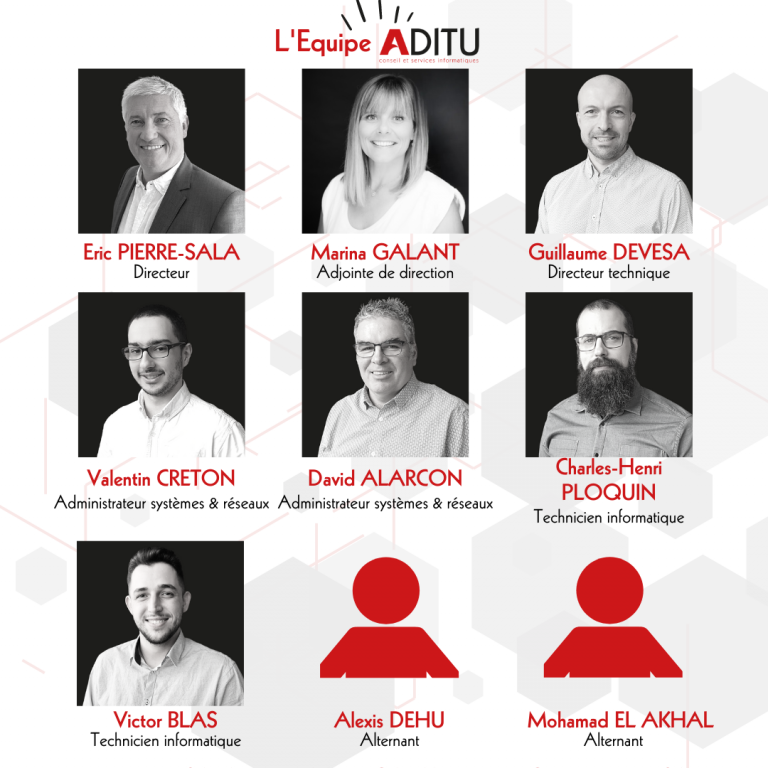
\includegraphics[scale = 0.5]{images/equipe_aditu.png}
  \caption{Membres de l'équipe d'ADITU lors mon alternance.}  
  \label{fig:aditu_members} % pour la citer après
\end{figure}

\subsection{Secteur d'activité professionnel}

Le secteur d'activité d'ADITU se caractérise par la réponse aux besoins d'aider les entreprises du secteur à se développer en les déchargeant de l'élaboration ou du maintient de leur infrastructure informatique. ADITU tend à être l'intermédiaire des professionnels locaux au monde du numérique.
\\ \\
ADITU permet à ses clients de pouvoir se concentrer sur leurs activités professionnelles en les déchargeant de l'utilisation d'une infrastructure faillible, vieillissante ou incorrectement maintenue (pertes de données, complexité à l'utilisation, problème d'expansibilité, failles de sécurités...).  
\\ \\
Le secteur d'activité est solide, assurant aux entreprises leur bon fonctionnement sans qu'elles aient besoin de recruter et de former une unique personne pour maintenir leurs infrastructures. L'équipe d'ADITU travaille à la performance et à la refocalisation des entreprises sur leurs activités.

\subsection{Clientèle ciblée et ses besoins}

ADITU a été fondé en soutient aux entreprises du Pays Basque, des Landes et du Béarn. Sa zone d'attractivité s'étend dans ces régions. Cette zone de chalandise reste locale mais très éclatée sur la côte Basque. Le Directeur M. Éric Pierre-Sala souhaite que l'entreprise garde cette proximité avec ses clients et ses acteurs pour conserver une relation humaine force d'ADITU.
\\ \\
La clientèle ciblée est variée, regroupant entreprises et organisations locales ayant besoin d'externaliser tout ou partie de la gestion de leur infrastructure à de grands groupes souhaitant s'installer dans le Pays Basque. La plupart des clients d'ADITU sont des clients historiques de toute taille avec au moins de dix années d'ancienneté.
\\ \\
Les clients d'ADITU sont des clients souhaitant de la proximité et de l'humain pour leur informatique, pouvant communiquer rapidement avec une personne ou son équipe. Ces personnes sont souvent rattachées à leur région par leur activité économique ou commerciale, et sont demandeurs d'acteurs locaux.

\subsection{Services distribués}

Pour répondre aux besoins du secteur, ADITU propose des services de conseils, d'installation et de maintenance d'infrastructures informatiques à la demande. Chaque client peut choisir la souscription d'un ou plusieurs services selon leurs besoins et le support souhaité.
\\ \\
Pour assurer la continuité des services proposés, ADITU possède deux data centres \textit{(Centres d'hébergement et de Gestion des données)} à Bidart et à Dax. Ces data centres servent à \textbf{l'hébergement} de machines dédiées aux clients ou à l'hébergement de leurs services que nous maintenons continuellement (sites WEB, messagerie, stockage et partage de fichiers, systèmes de sauvegardes, applications métier...).
\\ \\
ADITU propose aussi la supervision du fonctionnement de ces services, hébergés en data centres ou sur les sites des clients. Le service \textbf{d'infogérance} permet aux clients d'être informés en tant réel de la disponibilité de leurs services pour leurs collaborateurs, et d'être rassurés de leur remise en fonctionnement et de leur suivi. L'infogérance englobe le support téléphonique et informatique, l'aide à la résolution de problèmes quotidien, les interventions éventuelles et une astreinte.
\\ \\
Des journées en \textbf{régie} sont proposées, permettant l'envoi d'un technicien dédié au support et au contrôle du bon fonctionnement de l'infrastructure sur l'ensemble d'une journée. Le technicien est alors sollicité pour des problèmes mineurs, des formations, de l'installation de matériel ou autre. Ce type de journées est intéressant pour la vérification d'une utilisation propre de l'infrastructure installée et pour faciliter l'activité du client.

\subsection{Organisation des équipes}

Côté organisationnel, l'équipe technique se réunit chaque lundi matin avec le dirigeant de l'entreprise pour planifier les actions de la semaine suivant les retours et les appels des clients, afin de planifier des journées en régie ou autres activités de la semaine. Cette réunion est dite d'exploitation.
\\ \\
Cette réunion est suivie d'un point technique sous la conduite du directeur technique, commun à toute l'équipe technique où sont discutés les progrès des semaines précédentes avec leurs potentiels points bloquants, puis de la méthodologie d'approche du travail de la semaine défini dans la réunion d'exploitation. Le tout sous conseil et la supervision de l'ensemble de l'équipe.
\\ \\
Plusieurs réunions, points ou comités peuvent être organisés dans la semaine, planifiés lors de la réunion d'exploitation de la semaine ou plusieurs semaines à l'avance.
\\ \\
Chaque jour, une personne est aussi dite de support, travaillant sur ses projets et répondant aux demandes de support des clients. Cela permet à tous les membres de l'équipe de pouvoir se consacrer à leurst projets sans devoir penser à répondre constamment aux appels.

\newpage